\documentclass{beamer}

\usepackage[utf8]{inputenc}
\usepackage[czech]{babel}
\usepackage[normalem]{ulem}

\usetheme{Blacko}

\setcounter{tocdepth}{2}  % hide subsubsections and lower

\AtBeginSection[]{
	\ifnum \value{framenumber}>1  % don't show on first page
		\begin{frame}
			\frametitle{Plan}
			\tableofcontents[currentsection]
		\end{frame}
    \else\fi

	\begin{frame}
	\vfill
	\begin{beamercolorbox}[sep=8pt,center,shadow=true,rounded=true]{title}
		\usebeamerfont{title}\insertsectionhead\par%
	\end{beamercolorbox}
	\vfill
	\end{frame}	    
}

\AtBeginSection[]{
	\begin{frame}
	\vfill
	\begin{beamercolorbox}[sep=8pt,center,shadow=true,rounded=true]{title}
		\usebeamerfont{title}\insertsectionhead\par%
	\end{beamercolorbox}
	\vfill
	\end{frame}	    
}
  
\setbeamercovered{%
  again covered={\opaqueness<1->{15}}}

\title{\texttt{\LARGE Dvoukanálový USB osciloskop}}
\subtitle{ Obhajoba DMP }
\author{ Adam Verner\footnote{\texttt{vernead15@sps-prosek.cz}}}

\begin{document}

\begin{frame}
  \maketitle \\
\end{frame}


\begin{frame}{Jak jsem na tom?}
	\begin{itemize}
		\item Součástky už jsem obědnal z AliExpressu
		\item Vlastně stačí jenom doprogramovat a doladit
		\item O jarních prázdnínách obědnám plošňák z číny
		\item Vše vytisknu na 3D tiskárně
	\end{itemize}
\end{frame}


\begin{frame}{konec}
	\Huge Děkuji za pozornost. \\[.35cm]
	\normalsize otázky?
\end{frame}

\begin{frame}{Co nás v prezentaci čeká?}
  \tableofcontents
\end{frame}
	
\section{Hardware}

	\subsection{Krabička}
	\begin{frame}{krabičku}
		\centering
		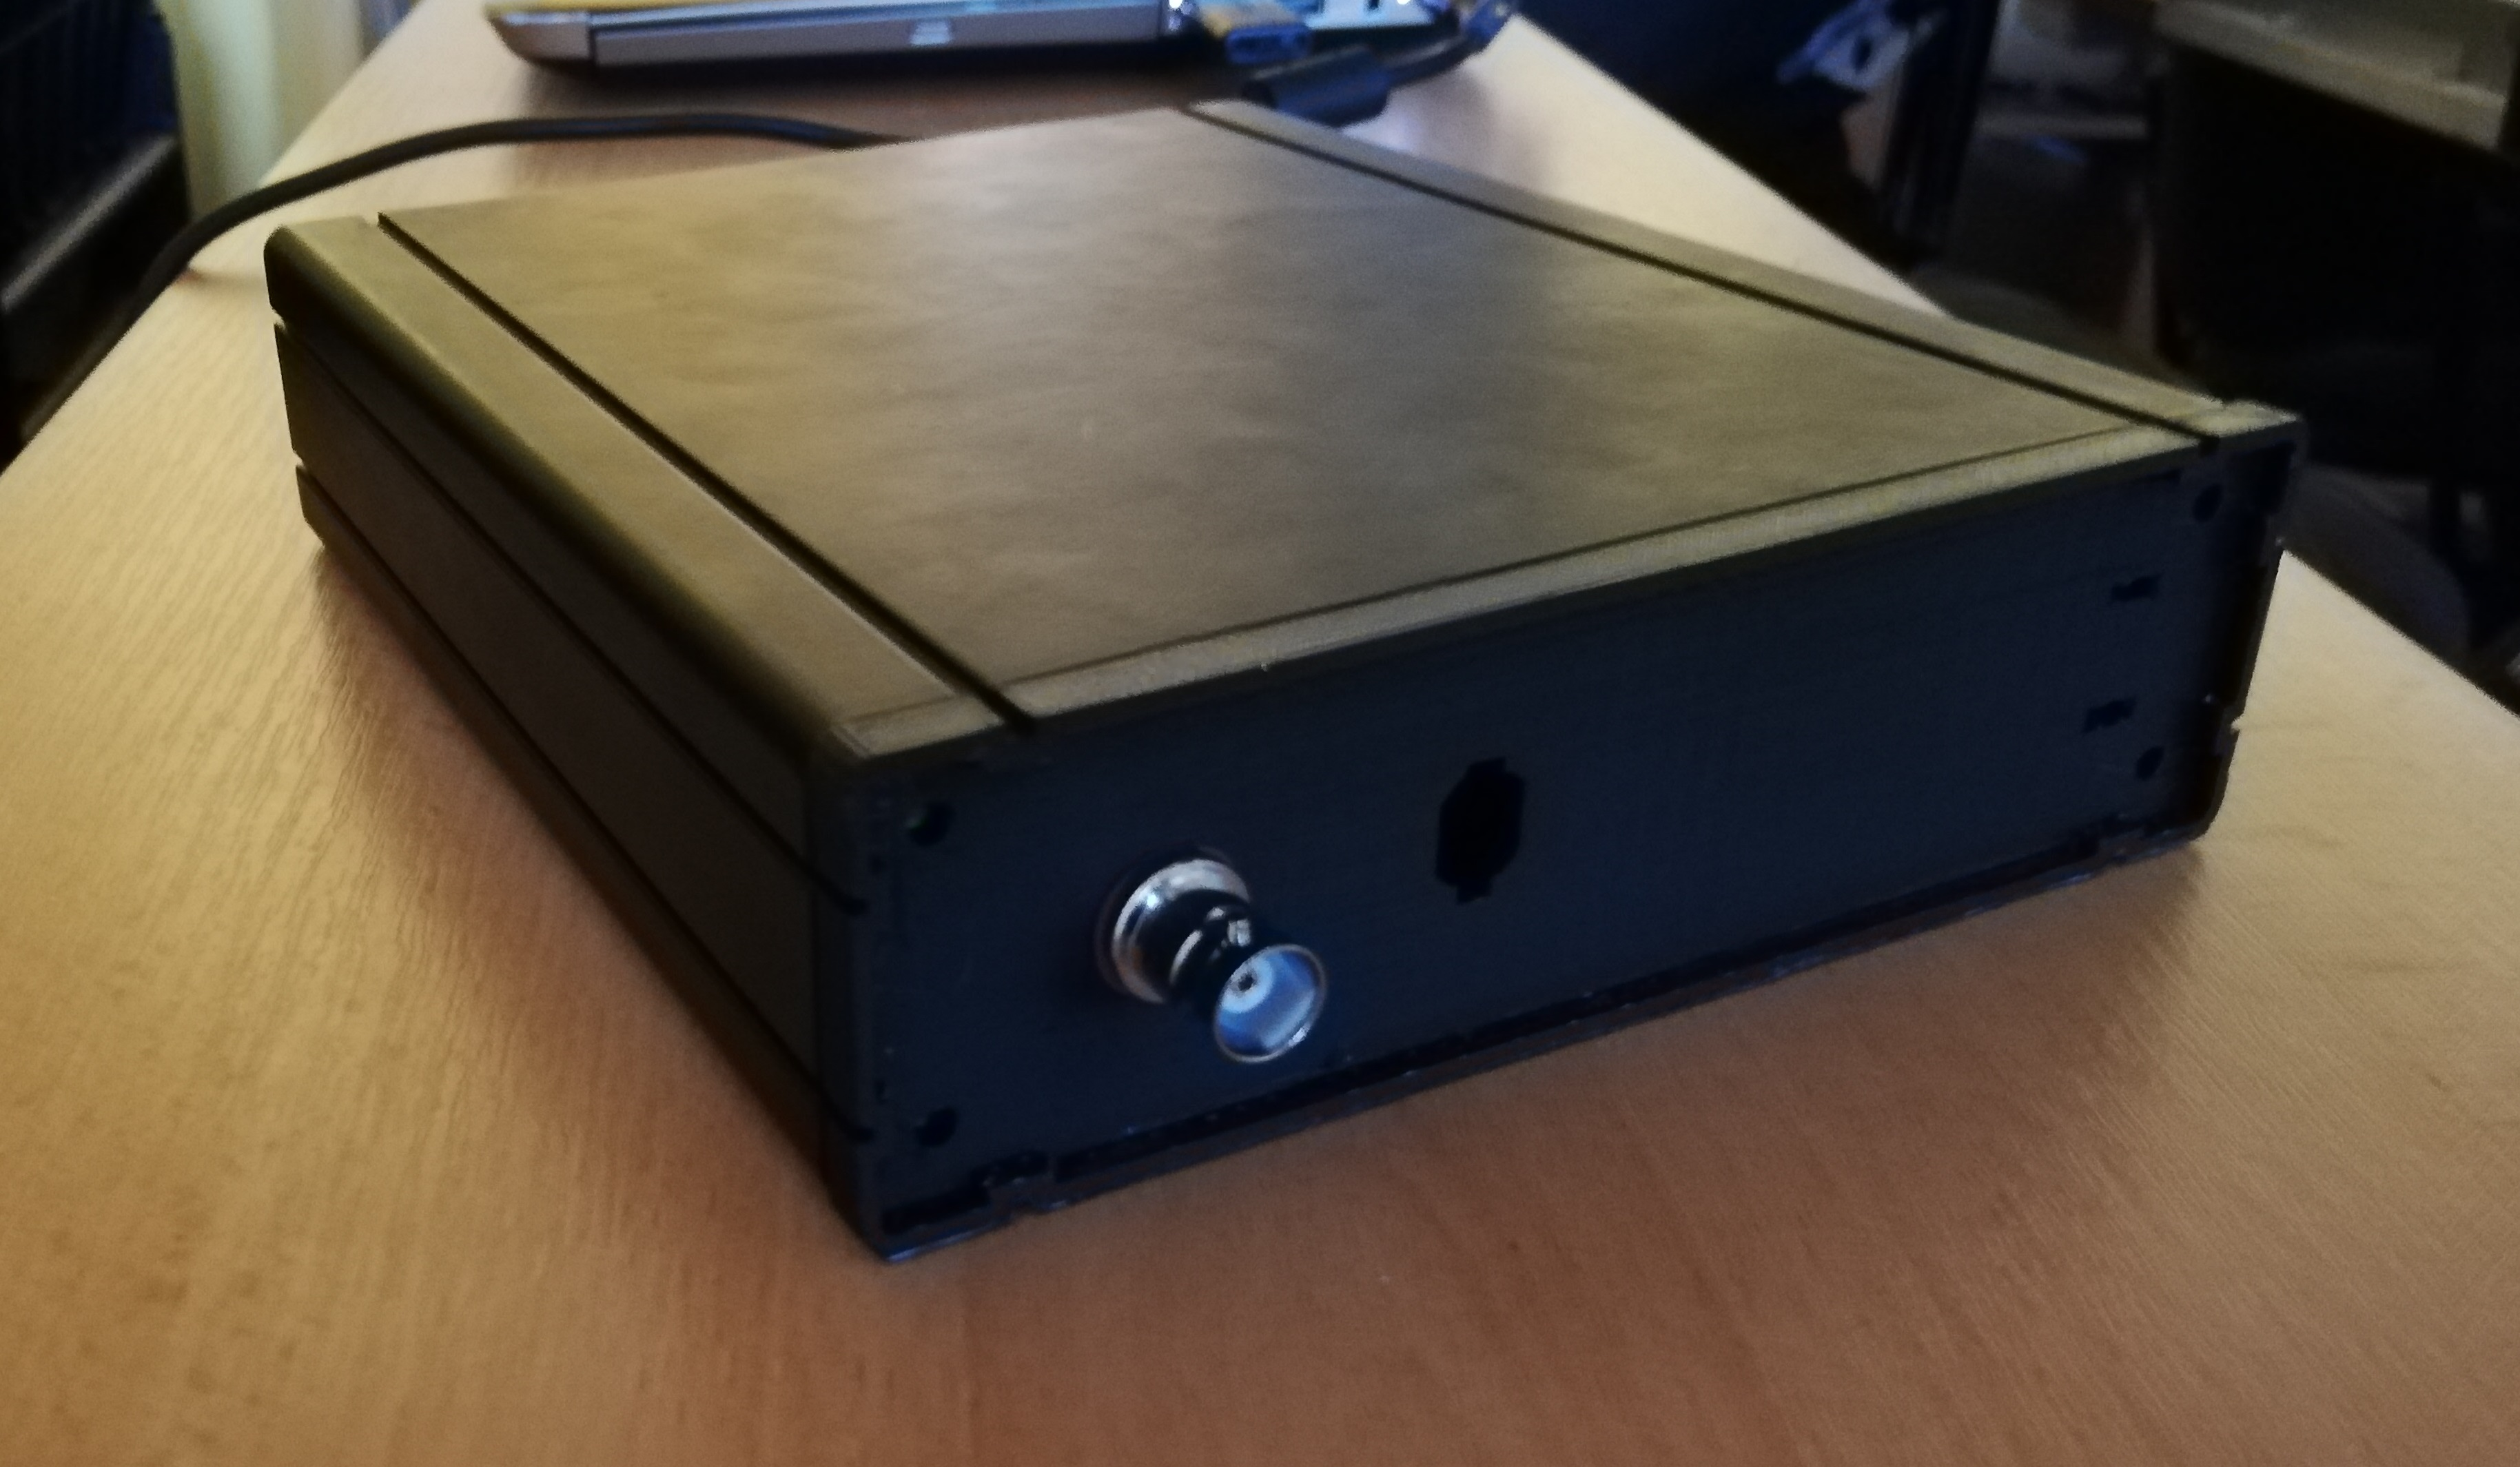
\includegraphics[width=\linewidth]{outer_profile.jpg}
	\end{frame}		
	
	\subsection{Destičky}
	\begin{frame}{}
		\centering
		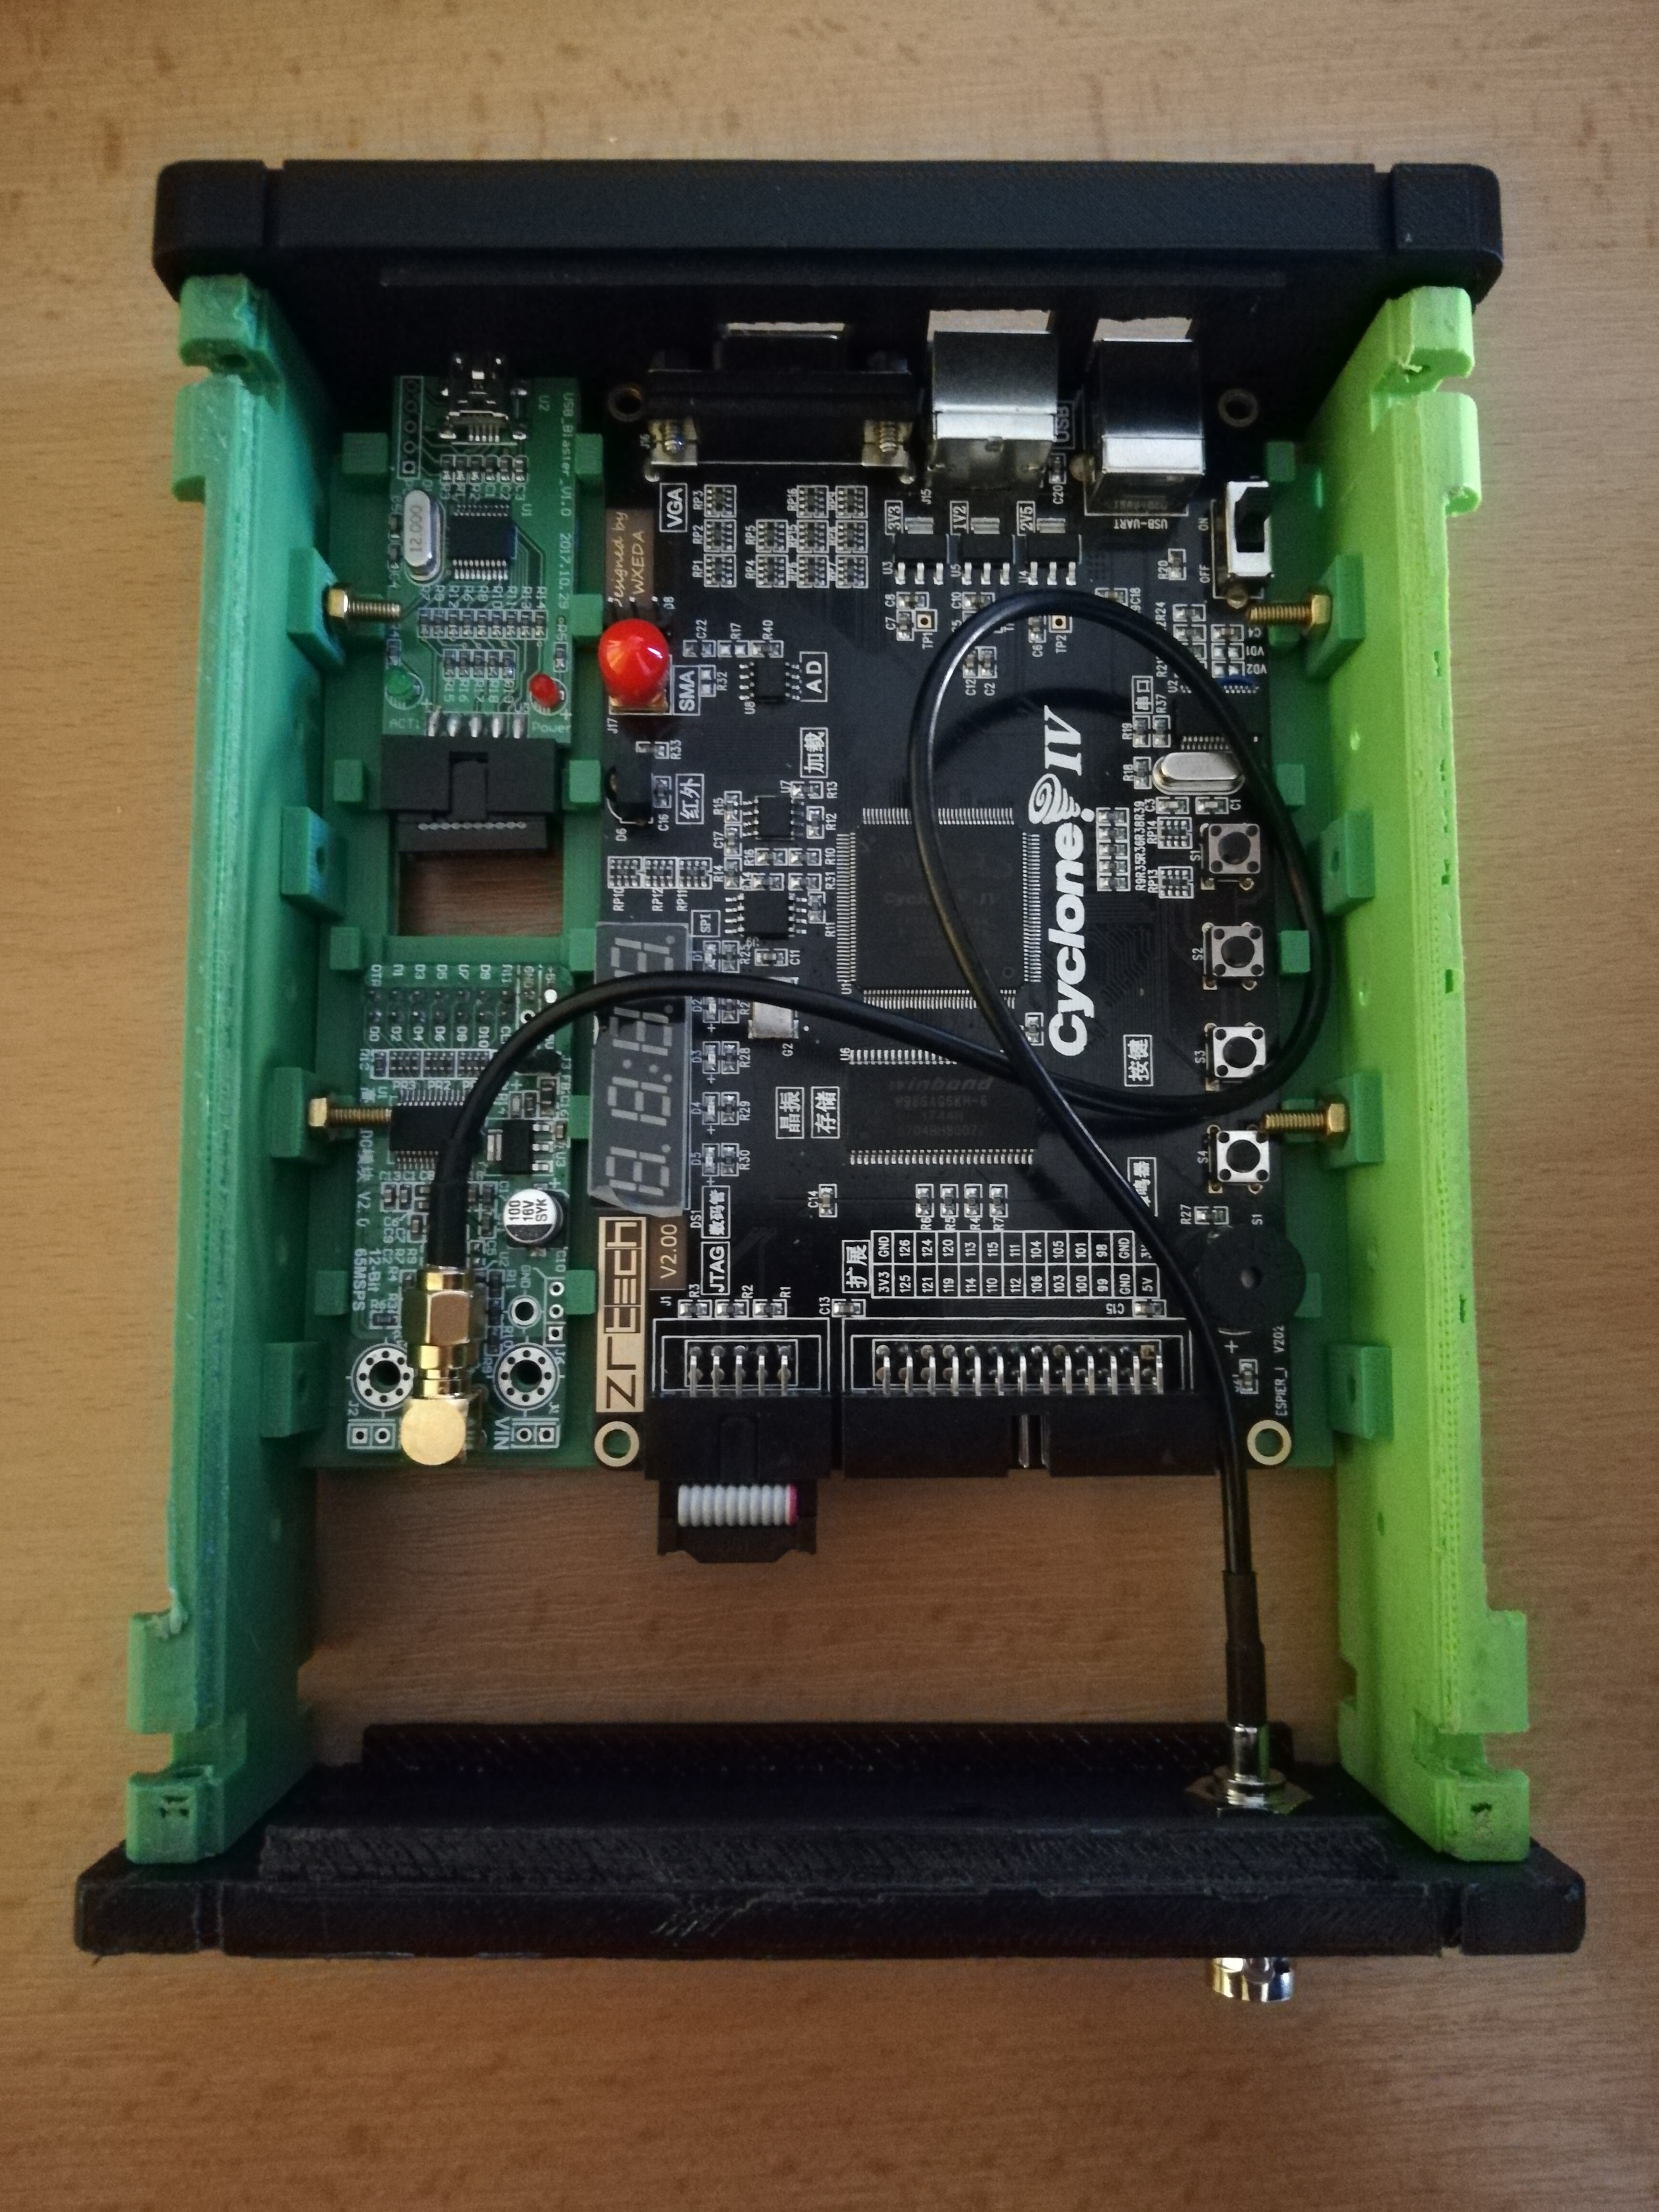
\includegraphics[height=0.90\paperheight]{intensities.jpg}
	\end{frame}
	
\section{Software}

	\subsection{Design}
		\begin{frame}{Software}
			\centering
			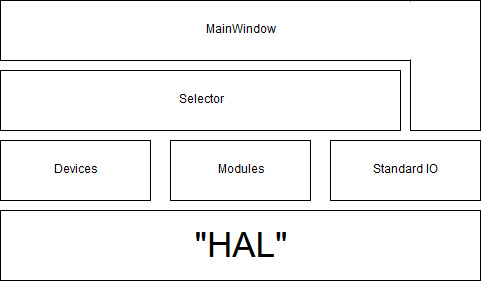
\includegraphics[width=\linewidth]{software_layers.jpg}
	\end{frame}

	\subsection{screenshot}
		\begin{frame}{Software}
			\centering
			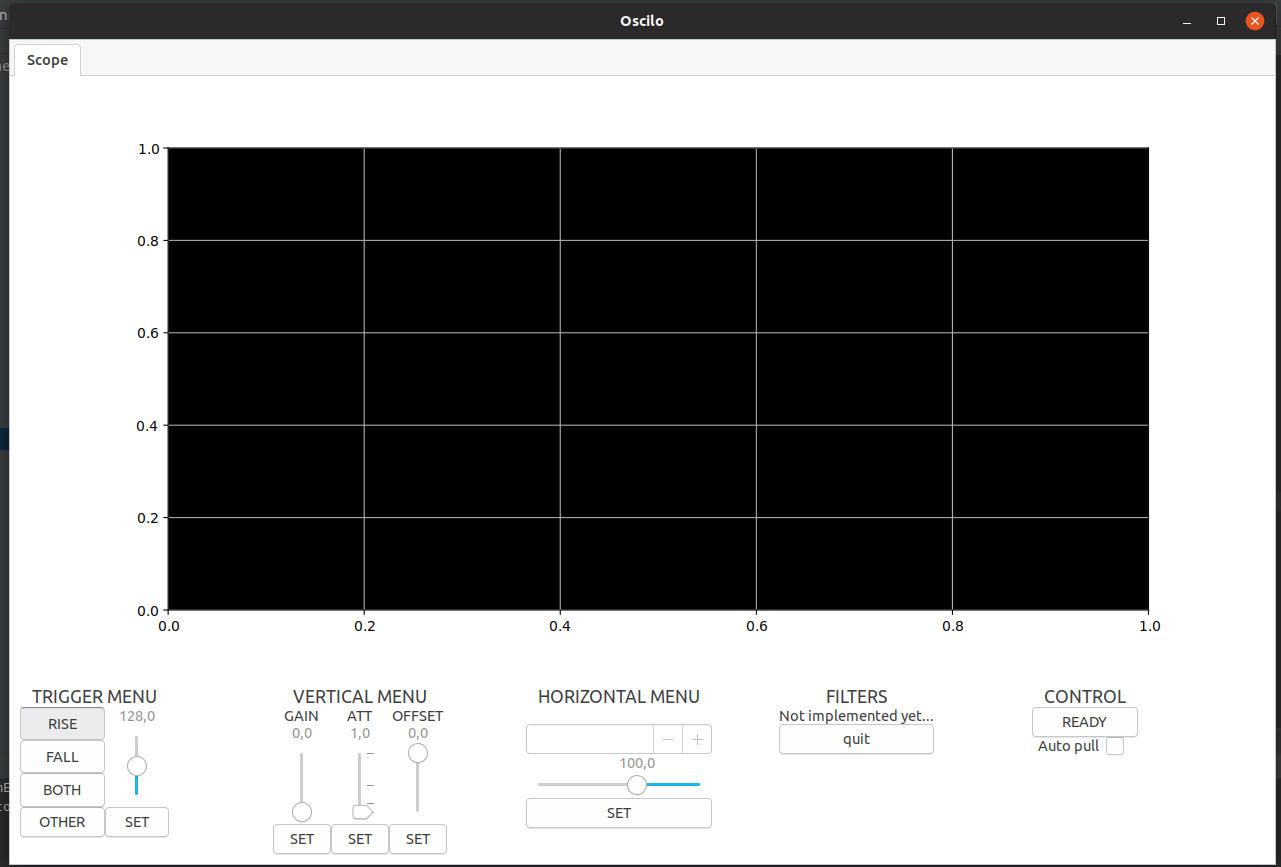
\includegraphics[width=0.95\linewidth]{oscilo_fake.png}
		\end{frame}
	\subsection{backend}	
		\begin{frame}{Software}
			\centering
			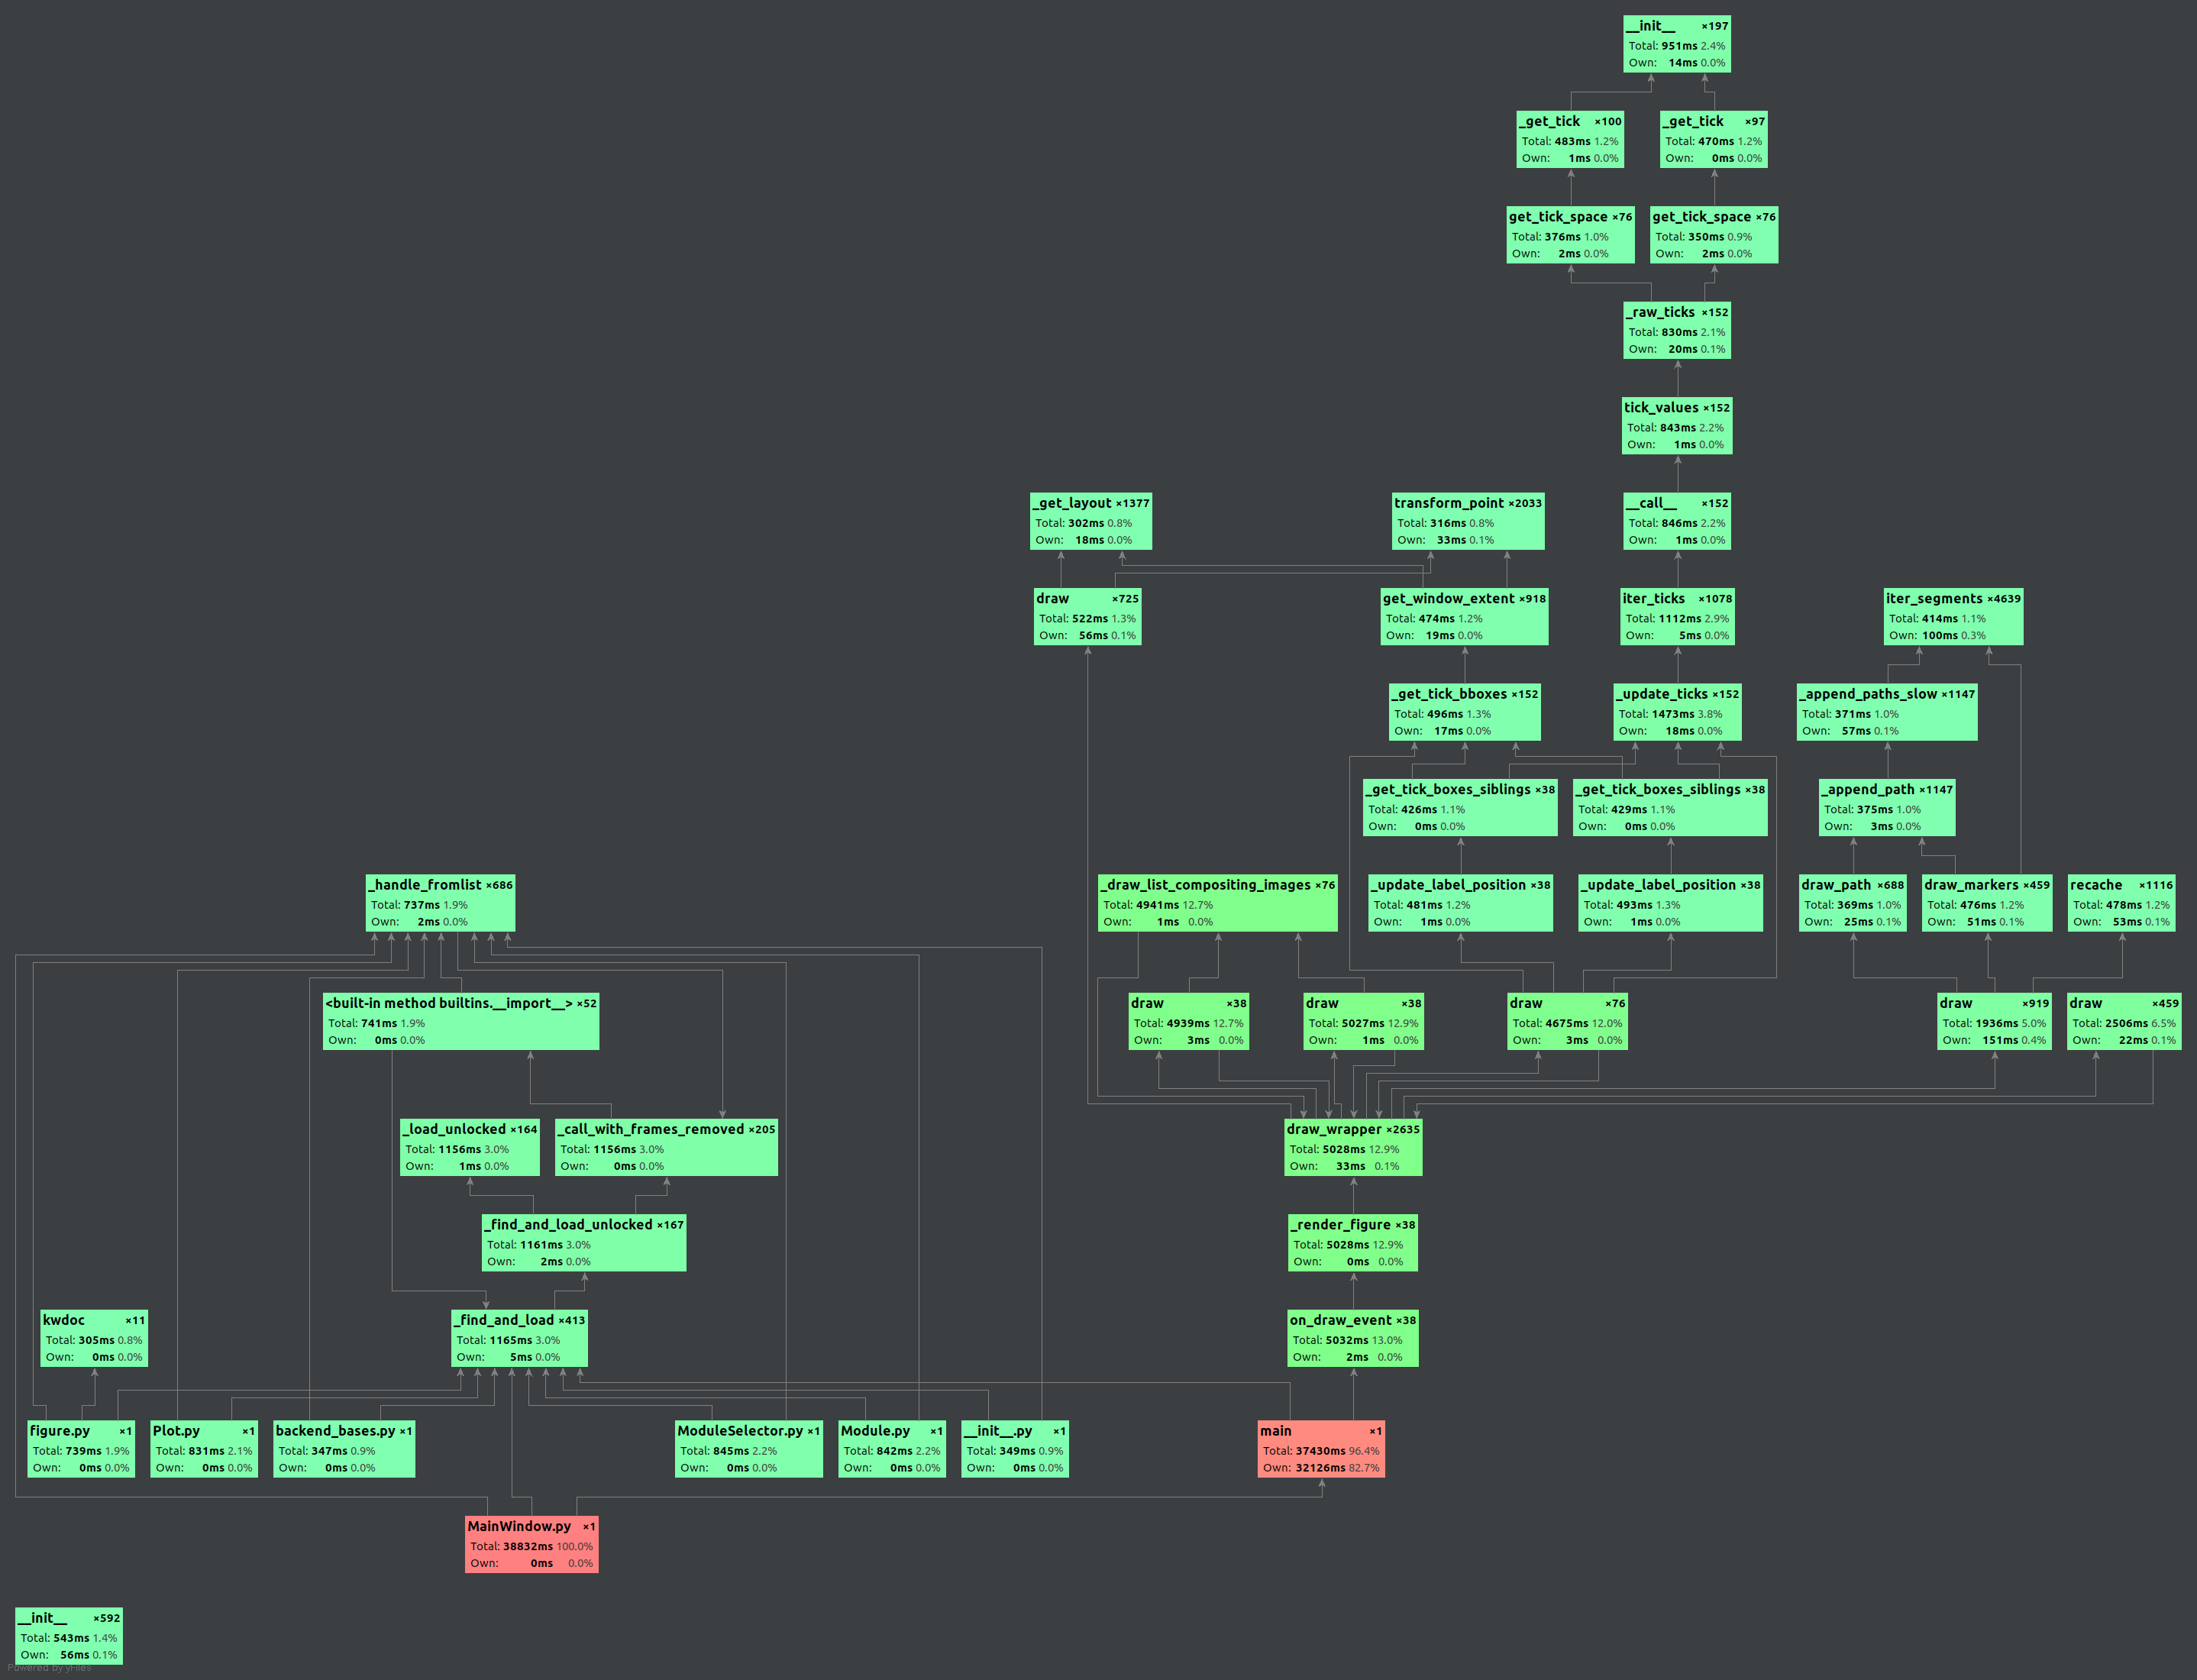
\includegraphics[width=\linewidth]{profile_fake.png}
		\end{frame}
	
\section{Firmware}
	\subsection{Module}
		\begin{frame}{Software}
			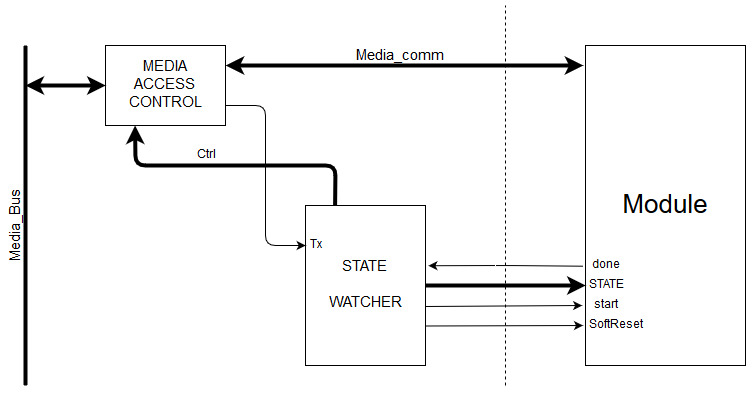
\includegraphics[width=\linewidth]{module.jpg}
		\end{frame}
	\subsection{RTL}	
		\begin{frame}{Software}
			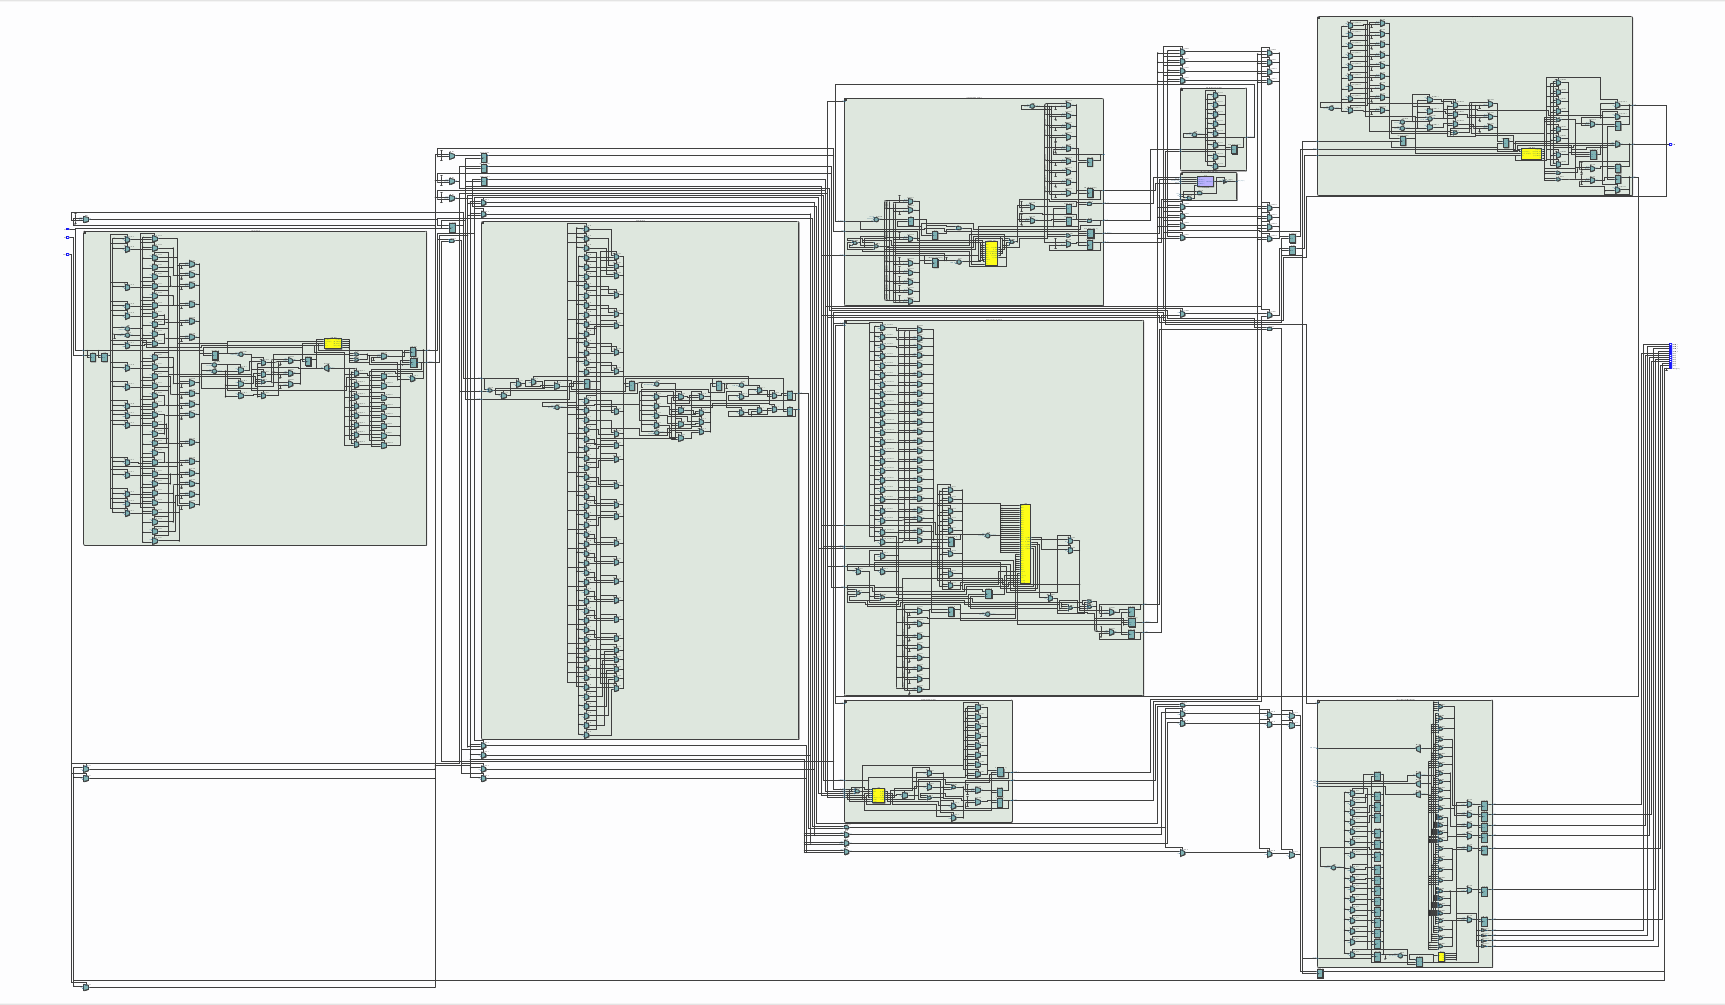
\includegraphics[width=\linewidth]{rtl_fake.png}
		\end{frame}
	
	
\section{Docs}

	\subsection{LaTeX}
		\begin{frame}{LaTeX}
			
		https://github.com/AdamVerner/SPSProsekDMPTemplate
			
		\end{frame}


\end{document}
\endinput

